% Volume II: Calculus, Analysis, and Continuous Mathematics
% Continuity note for Chapter 8.
% Previous dependencies: Chapters 1 and 2 introduced typed functions, domains, codomains, and notation discipline; Chapters 3-5 introduced norms, distances, linear approximation geometry, projections, and residuals; Chapters 6-7 prepare the idea that preferred directions, tensors, and array computations need derivatives and local linear maps.
% New durable concepts: limits; one-sided limits; continuity; epsilon-delta stability; derivatives as limits and local linear maps; differentials; product and chain rules; Riemann sums; definite integrals; accumulation functions; the fundamental theorem of calculus; ordinary differential equations; initial conditions; equilibria; Euler simulation.
% Forward hooks: Chapter 9 turns derivatives into gradients, Jacobians, and Hessians for many variables; Chapter 10 uses Taylor approximation as a local modeling rule; Chapter 11 uses integrals for densities and change of variables; Chapter 12 uses integrals and differential equations for signals and operators; Chapters 13-18 reuse continuity, integration, and approximation in probability, expectation, inference, and information.
% Notation commitments: Scalar inputs use x,a,h; scalar functions are f:D\subseteq\mathbb{R}\to\mathbb{R}; limits use \lim_{x\to a}f(x)=L and one-sided variants; derivatives use f'(a) and the differential df_a(h)=f'(a)h; rates use r(t); integrals use \int_a^b r(t)\,dt; ODE states use x(t), \dot x(t), initial value x(t_0)=x_0, and Euler steps x_{k+1}=x_k+\Delta t f(x_k,t_k).
% Figure plan: four ImageGen raster figures are used and referenced: limits and continuity for 8.1; tangent/local linearization for 8.2; Riemann accumulation for 8.3; ODE trajectory and Euler steps for 8.4.
\section{Chapter 8: Limits, Continuity, Derivatives, and Integrals}
\label{ch:limits-continuity-derivatives-integrals}

The first volume built a finite-dimensional language for objects, maps, vectors, matrices, projections, spectra, and tensor-shaped computations. That language is exact, but many scientific and learning problems ask how quantities change when an input is nudged, when time advances a little, or when many tiny contributions are accumulated into a macroscopic quantity. Calculus is the mathematics of those controlled transitions.

This chapter rebuilds elementary calculus around two habits that will matter throughout computational neuroscience and AI. First, a complicated object can often be understood by a nearby simpler object: a limiting value, a tangent line, or a local linear map. Second, a large quantity can often be built by adding many small pieces: a total spike count, an area under a loss curve, an expected value, or the trajectory of a dynamical system.

\paragraph{Chapter problem.}
How do we make precise statements about nearby behavior, replace nonlinear change by local linear change, and accumulate infinitesimal pieces into totals or trajectories?

\paragraph{Section map.}
Section 8.1 defines limits and continuity as stable behavior under small input changes. Section 8.2 defines the derivative as a limit and interprets it as the best local linear approximation. Section 8.3 defines integrals as accumulated quantities and proves the link between accumulation and derivatives. Section 8.4 previews differential equations, where local rates are stitched together into continuous-time dynamics.

\subsection{8.1 Limits and continuity}

\paragraph{Motivating question.}
When inputs get arbitrarily close to \(a\), what value, if any, must the outputs \(f(x)\) get close to?

\paragraph{Beginner setup.}
A \emph{limit} describes what a function approaches near an input, not necessarily what the function equals at that input. If
\[
\lim_{x\to a} f(x)=L,
\]
then values of \(f(x)\) can be forced as close to \(L\) as desired by taking \(x\) close enough to \(a\), with \(x\neq a\). A function is \emph{continuous} at \(a\) when the limiting value and the actual value agree:
\[
\lim_{x\to a}f(x)=f(a).
\]

The smallest nontrivial example is
\[
f(x)=\frac{x^2-1}{x-1},\qquad x\neq 1.
\]
For every \(x\neq 1\),
\[
f(x)=x+1,
\]
so as \(x\) approaches \(1\), \(f(x)\) approaches \(2\). The limit is \(2\), even though the displayed fraction is not defined at \(x=1\). If we define \(f(1)=2\), the hole is filled and the function becomes continuous at \(1\). If we define \(f(1)=0\), the limit is still \(2\), but the function is not continuous at \(1\).

Limits solve the problem of describing behavior near a point when direct substitution is unavailable or misleading. Continuity solves the stability problem: small changes in input should produce small changes in output.

What to keep in mind: a limit is a statement about all sufficiently nearby inputs, not about a single sample point. Continuity adds the requirement that the function's actual value at the point matches the nearby behavior.

\begin{figure}[htbp]
\centering
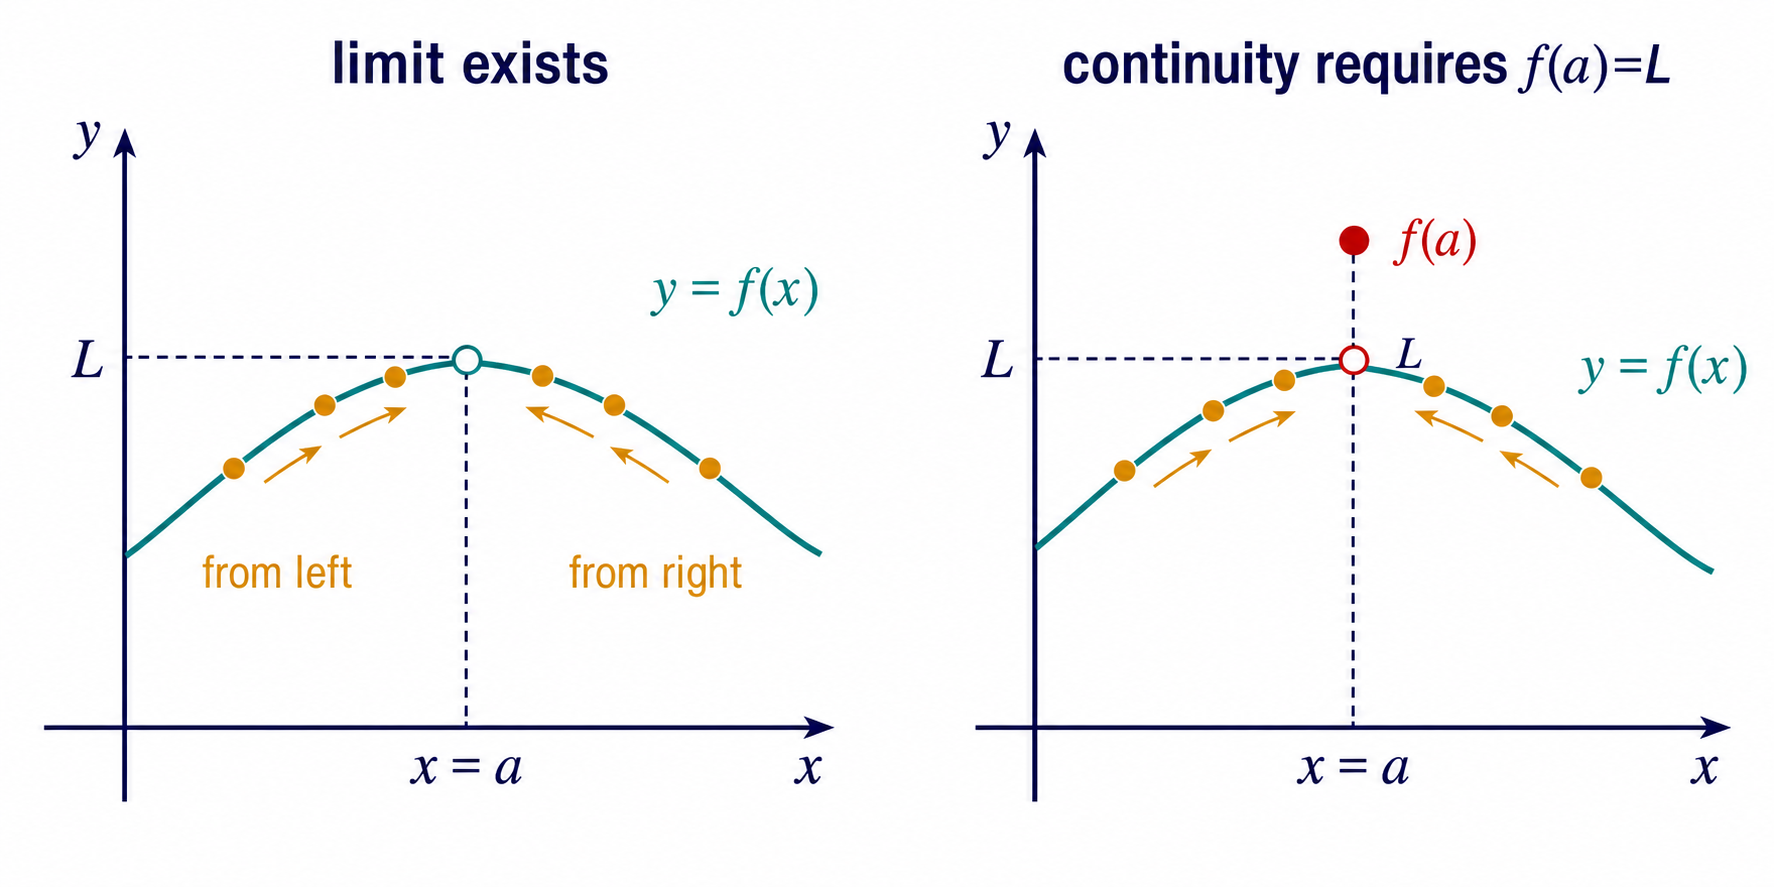
\includegraphics[width=0.95\linewidth]{imagegen-figures/ch08-limits-continuity.png}
\caption{A limit is about approach, while continuity also checks the actual value. In the left panel, values from both sides approach the same height \(L\) as \(x\to a\). In the right panel, the nearby values still approach \(L\), but the solid point \(f(a)\) is elsewhere, so the function is not continuous at \(a\).}
\label{fig:ch08-limits-continuity}
\end{figure}

\paragraph{Formal setup.}
Let \(D\subseteq\mathbb{R}\), let \(f:D\to\mathbb{R}\), and let \(a\) be a point that can be approached by points of \(D\) other than \(a\). We write
\[
\lim_{x\to a} f(x)=L
\]
if, for every tolerance \(\varepsilon>0\), there exists a distance \(\delta>0\) such that
\[
x\in D,\quad 0<|x-a|<\delta
\qquad\Longrightarrow\qquad
|f(x)-L|<\varepsilon.
\]
The domain \(D\) matters: it tells us which inputs are allowed to approach \(a\).

The \emph{right-hand limit} is
\[
\lim_{x\to a^+}f(x)=L,
\]
where only inputs \(x>a\) are allowed. The \emph{left-hand limit} is
\[
\lim_{x\to a^-}f(x)=L,
\]
where only inputs \(x<a\) are allowed. A two-sided limit exists exactly when both one-sided limits exist and are equal.

The function \(f\) is \emph{continuous at \(a\in D\)} if
\[
\lim_{x\to a}f(x)=f(a).
\]
It is continuous on a set \(S\subseteq D\) if it is continuous at every point of \(S\), using one-sided continuity at endpoints when the domain has endpoints.

\paragraph{Core intuition.}
Figure~\ref{fig:ch08-limits-continuity} separates two ideas that beginners often merge. Nearby values may settle toward \(L\), even if the function is undefined at \(a\) or assigned the wrong value there. The phrase "as \(x\to a\)" asks us to watch a process of approach. It does not say "plug in \(a\)".

The epsilon-delta definition is a stability contract. The output tolerance \(\varepsilon\) is chosen first: "I want \(f(x)\) within this much of \(L\)." The definition says that there must be an input tolerance \(\delta\): "then it is enough to keep \(x\) within this much of \(a\), excluding \(a\) itself." Continuity is the special case where the target output is the actual value \(f(a)\).

Common misconceptions are predictable. First, a limit can exist even if \(f(a)\) is undefined. Second, a limit can fail even if \(f(a)\) is defined, as with a jump discontinuity. Third, checking a few numerical inputs near \(a\) can suggest a limit, but it does not prove one. Fourth, continuity is local: a function can be continuous at one point and discontinuous at another.

This section extends the function notation from Chapter 2 and the distance language from Chapter 3. It prepares derivatives, optimization stability, numerical analysis, and probability densities, where small perturbations should not arbitrarily change predictions or accumulated probabilities.

\paragraph{Main theorem: continuity preserves limits of sequences.}
Let \(f:D\to\mathbb{R}\) and \(a\in D\). The function \(f\) is continuous at \(a\) if and only if, for every sequence \((x_n)\) in \(D\) with \(x_n\to a\), we have
\[
f(x_n)\to f(a).
\]

\emph{Proof sketch.} Suppose first that \(f\) is continuous at \(a\). Choose any sequence \(x_n\to a\). To prove \(f(x_n)\to f(a)\), start with an output tolerance \(\varepsilon>0\). Continuity gives a \(\delta>0\) such that
\[
|x-a|<\delta \quad\Longrightarrow\quad |f(x)-f(a)|<\varepsilon.
\]
Because \(x_n\to a\), there is an index \(N\) such that \(n\geq N\) implies \(|x_n-a|<\delta\). Therefore \(n\geq N\) implies \(|f(x_n)-f(a)|<\varepsilon\), which is exactly \(f(x_n)\to f(a)\).

For the converse, argue by contradiction. If \(f\) is not continuous at \(a\), then there is some output tolerance \(\varepsilon_0>0\) such that no matter how small a \(\delta\) is chosen, we can find \(x\in D\) with \(|x-a|<\delta\) but
\[
|f(x)-f(a)|\geq \varepsilon_0.
\]
Choose \(\delta=1/n\) for \(n=1,2,\dots\), and pick such a point \(x_n\). Then \(x_n\to a\), but \(f(x_n)\) does not approach \(f(a)\), contradicting the sequence condition. Thus the sequence condition is equivalent to continuity.

\paragraph{Worked examples.}
\emph{Small symbolic example.} Let
\[
f(x)=
\begin{cases}
x+1, & x\neq 1,\\
0, & x=1.
\end{cases}
\]
As \(x\to 1\), the expression \(x+1\) approaches \(2\), so
\[
\lim_{x\to 1} f(x)=2.
\]
But \(f(1)=0\). Therefore \(f\) is not continuous at \(1\). If we changed only the value at \(1\) to \(f(1)=2\), the new function would be continuous at \(1\).

\emph{ML/neuroscience example.} A soft threshold firing-rate model might use
\[
r(s)=\frac{1}{1+\exp(-10(s-0.2))},
\]
where \(s\) is stimulus strength and \(r(s)\) is a normalized firing rate. This function is continuous: a tiny change in \(s\) changes \(r(s)\) only slightly. A hard threshold model
\[
h(s)=
\begin{cases}
0, & s<0.2,\\
1, & s\geq 0.2
\end{cases}
\]
has a jump at \(s=0.2\). The right-hand limit is \(1\), the left-hand limit is \(0\), and the two-sided limit does not exist. The hard threshold may be useful as an idealization, but it predicts an abrupt output change from an arbitrarily small input perturbation.

\paragraph{ML/DL/neuroscience connections.}
Continuity is a minimal mathematical version of robustness. In machine learning, a continuous model cannot jump infinitely under an infinitesimal input perturbation, though it can still be very steep. In deep learning, common operations such as affine maps, sigmoid, tanh, softmax, and ReLU are continuous, while some decision rules such as argmax are discontinuous. In neuroscience, continuous tuning curves support stable stimulus-response models, whereas discontinuities often signal an idealized decision boundary, threshold, or regime switch rather than a literal biophysical law.

\paragraph{Exercises.}
\begin{enumerate}[label=\textbf{8.1.\arabic*.}, leftmargin=*]
\item \textbf{Mechanical.} For \(f(x)=(x^2-4)/(x-2)\), \(x\neq 2\), compute \(\lim_{x\to 2}f(x)\). If \(f(2)=5\), is \(f\) continuous at \(2\)?
\item \textbf{Proof or derivation.} Prove from the epsilon-delta definition that
\[
\lim_{x\to 3}(2x-1)=5.
\]
Given \(\varepsilon>0\), state a valid choice of \(\delta\).
\item \textbf{Numerical/computational.} Write pseudocode that samples \(f(x)=\sin x/x\) at \(x=10^{-1},10^{-2},\dots,10^{-6}\). What limiting value does this suggest near \(0\)? Why is this numerical evidence not a proof?
\item \textbf{Interpretation.} In a model \(r(s)\) mapping stimulus strength to firing rate, what does continuity at \(s=a\) mean experimentally?
\item \textbf{Debug the misconception.} A student says, "The limit at \(a\) is always \(f(a)\)." Give a counterexample and explain the difference between a limit and continuity.
\end{enumerate}

\subsection{8.2 Derivatives as local linearization}

\paragraph{Motivating question.}
Near a point \(a\), what linear function best predicts how \(f(x)\) changes when \(x\) is nudged?

\paragraph{Beginner setup.}
A \emph{derivative} measures local change. It begins with an average rate of change:
\[
\frac{f(a+h)-f(a)}{h}.
\]
This is the slope of the secant line through the points \(a\) and \(a+h\). If this average rate approaches a stable value as \(h\to 0\), that limiting value is the derivative \(f'(a)\). The derivative is the slope of the tangent line and the coefficient in the best local linear approximation:
\[
f(a+h)\approx f(a)+f'(a)h.
\]

For the smallest example, let \(f(x)=x^2\) and \(a=3\). Then
\[
\frac{f(3+h)-f(3)}{h}
=\frac{(3+h)^2-9}{h}
=\frac{6h+h^2}{h}
=6+h.
\]
As \(h\to 0\), the average rate approaches \(6\), so \(f'(3)=6\). Near \(x=3\),
\[
x^2\approx 9+6(x-3).
\]
At \(x=3.1\), this gives \(9.6\), while the exact value is \(9.61\).

Derivatives solve the problem of replacing nonlinear behavior by linear behavior at a chosen scale. The replacement is local: it works best for small \(h\).

What to keep in mind: a derivative is not only a formula-producing rule. It is a limit, a tangent slope, a local linear map, and a unit conversion from small input changes to small output changes.

\begin{figure}[htbp]
\centering
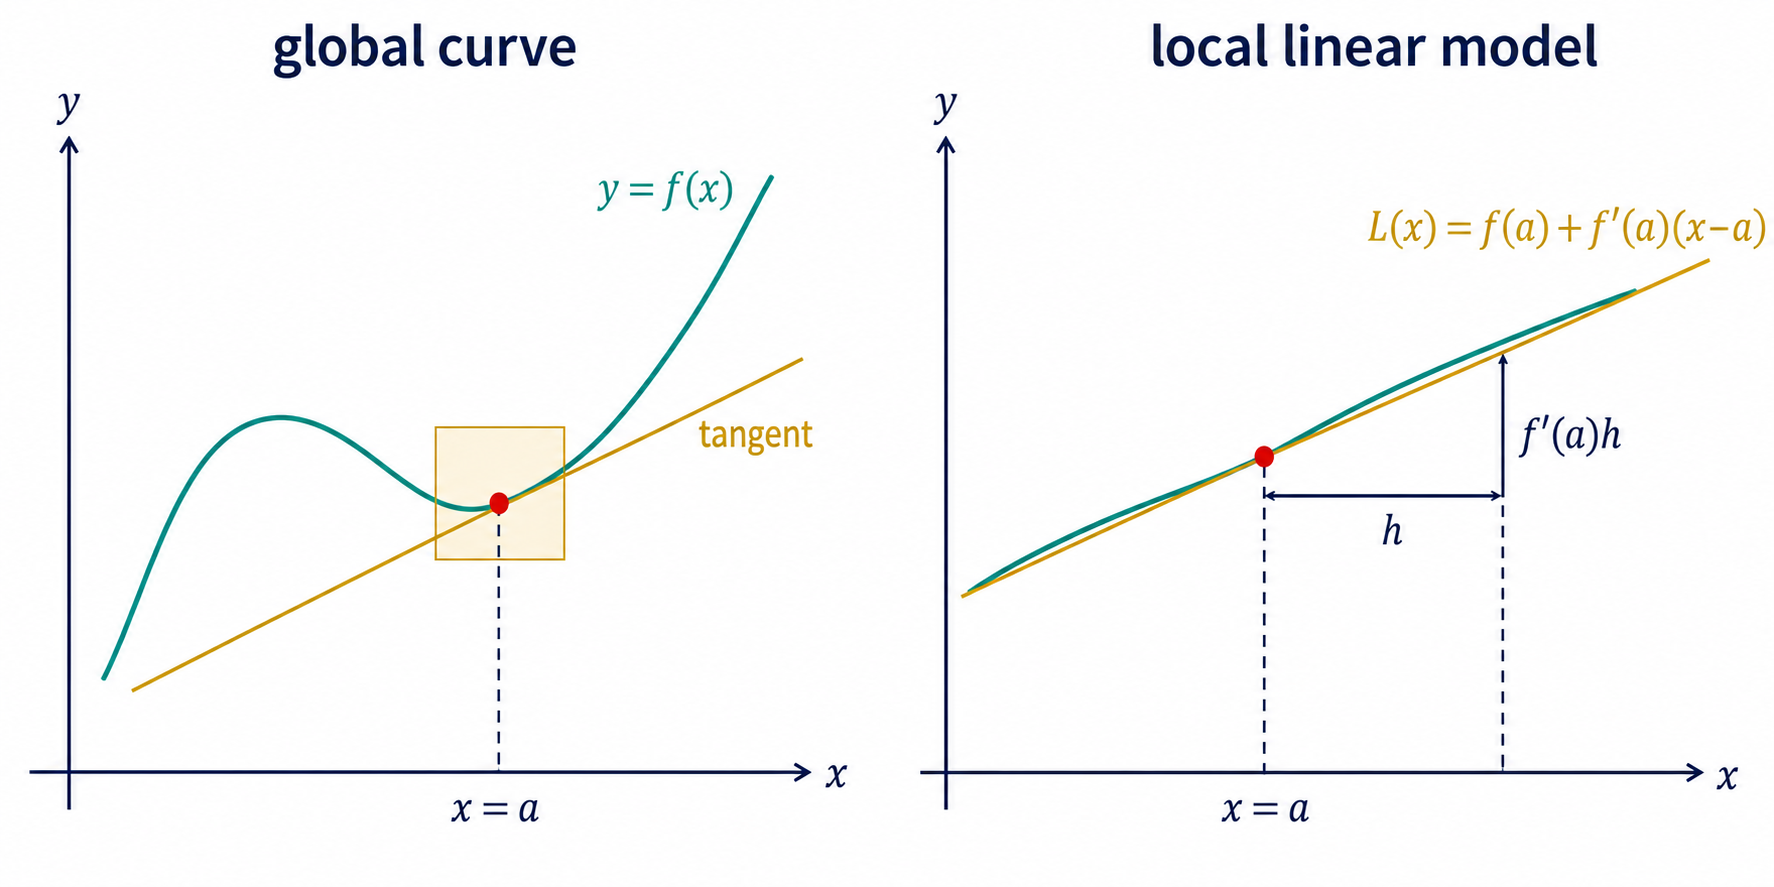
\includegraphics[width=0.95\linewidth]{imagegen-figures/ch08-derivative-local-linearization.png}
\caption{The derivative is the coefficient of the local linear model. Globally the curve bends, but after zooming near \(x=a\), the tangent line \(L(x)=f(a)+f'(a)(x-a)\) becomes a good replacement. A small input change \(h\) produces a first-order output change \(f'(a)h\).}
\label{fig:ch08-derivative-local-linearization}
\end{figure}

\paragraph{Formal setup.}
Let \(f:I\to\mathbb{R}\), where \(I\subseteq\mathbb{R}\) is an interval, and let \(a\) be an interior point of \(I\). The derivative of \(f\) at \(a\) is
\[
f'(a)=\lim_{h\to 0}\frac{f(a+h)-f(a)}{h},
\]
provided this limit exists. Equivalently, \(f\) is differentiable at \(a\) if there is a number \(m\) and an error term \(\rho(h)\) such that
\[
f(a+h)=f(a)+mh+\rho(h),
\qquad
\lim_{h\to 0}\frac{\rho(h)}{h}=0.
\]
Then \(m=f'(a)\). The linear map
\[
df_a:\mathbb{R}\to\mathbb{R},
\qquad
df_a(h)=f'(a)h,
\]
is the \emph{differential} of \(f\) at \(a\). This language connects one-variable calculus to the linear-map viewpoint from Chapter 4.

Derivative rules are shortcuts for limits. If \(f\) and \(g\) are differentiable at \(a\), then
\[
(f+g)'(a)=f'(a)+g'(a),
\]
\[
(fg)'(a)=f'(a)g(a)+f(a)g'(a),
\]
and, if \(g\) is differentiable at \(a\) and \(f\) is differentiable at \(g(a)\),
\[
(f\circ g)'(a)=f'(g(a))g'(a).
\]

\paragraph{Core intuition.}
Figure~\ref{fig:ch08-derivative-local-linearization} shows why derivatives belong in a course built around linear algebra. At a single point, a differentiable nonlinear function behaves like an affine map: base value plus linear change. If we subtract the base value \(f(a)\), the remaining first-order change is the linear map \(h\mapsto f'(a)h\).

The units matter. If \(t\) is measured in seconds and \(x(t)\) is measured in millivolts, then \(x'(t)\) has units millivolts per second. If a loss \(L(\theta)\) changes with a parameter \(\theta\), then \(L'(\theta)\) measures loss units per parameter unit. Derivatives are local conversion factors.

Common misconceptions include treating the derivative as a global slope, assuming differentiability wherever a graph is continuous, and forgetting that the approximation has an error term. The function \(f(x)=|x|\) is continuous at \(0\), but it is not differentiable at \(0\) because the left slope is \(-1\) and the right slope is \(1\). Smoothness is stronger than continuity.

This section turns the limit concept from Section 8.1 into a local replacement rule. Chapter 9 will extend \(df_a(h)=f'(a)h\) to gradients and Jacobians, where \(h\) is a vector and the derivative is a matrix-shaped linear map.

\paragraph{Main derivation: the chain rule from local linearization.}
Let \(g\) be differentiable at \(a\), and let \(f\) be differentiable at \(g(a)\). Write the small input change as \(h\). Differentiability of \(g\) gives
\[
g(a+h)=g(a)+g'(a)h+\rho_g(h),
\qquad
\frac{\rho_g(h)}{h}\to 0.
\]
Define the small output change of \(g\) by
\[
k=g(a+h)-g(a).
\]
Then \(k\to 0\) as \(h\to 0\), and differentiability of \(f\) at \(g(a)\) gives
\[
f(g(a)+k)=f(g(a))+f'(g(a))k+\rho_f(k),
\qquad
\frac{\rho_f(k)}{k}\to 0.
\]
Substitute \(k=g'(a)h+\rho_g(h)\):
\[
f(g(a+h))
=f(g(a))+f'(g(a))\bigl(g'(a)h+\rho_g(h)\bigr)+\rho_f(k).
\]
The coefficient of \(h\) in the first-order term is
\[
f'(g(a))g'(a).
\]
All remaining terms are small compared with \(h\). Therefore
\[
(f\circ g)'(a)=f'(g(a))g'(a).
\]
In words: the inner function converts an input perturbation \(h\) into an intermediate perturbation \(g'(a)h\), and the outer function converts that intermediate perturbation into an output perturbation \(f'(g(a))g'(a)h\).

\paragraph{Worked examples.}
\emph{Small numerical example.} Let \(f(x)=\sqrt{1+x}\), and approximate \(f(0.04)\) using the derivative at \(a=0\). Since
\[
f(0)=1,
\qquad
f'(x)=\frac{1}{2\sqrt{1+x}},
\qquad
f'(0)=\frac12,
\]
the local linear approximation is
\[
f(0+h)\approx 1+\frac12 h.
\]
With \(h=0.04\), this gives
\[
\sqrt{1.04}\approx 1.02.
\]
The exact value is approximately \(1.0198\), so the local linear model is accurate at this small scale.

\emph{ML/neuroscience example.} Consider a one-dimensional neural response nonlinearity
\[
r(s)=\sigma(2s-1),
\qquad
\sigma(z)=\frac{1}{1+e^{-z}}.
\]
At \(s=0.5\), the inner variable is \(z=0\), so \(\sigma(z)=0.5\) and \(\sigma'(z)=\sigma(z)(1-\sigma(z))=0.25\). By the chain rule,
\[
r'(0.5)=\sigma'(0)\cdot 2=0.5.
\]
A small stimulus change \(\Delta s=0.02\) therefore changes the firing-rate prediction by about
\[
\Delta r\approx 0.5(0.02)=0.01.
\]
Here the derivative is the local gain of the encoding model.

\paragraph{ML/DL/neuroscience connections.}
Backpropagation is repeated application of the chain rule through a computational graph. Each local derivative tells how a small change in one node affects a later node, and matrix calculus in Chapter 9 generalizes this to many coordinates at once. In optimization, the derivative of a loss tells which direction locally increases or decreases the loss. In neuroscience, derivatives describe gains of tuning curves, membrane-voltage rates, and sensitivities of decoder outputs to neural activity.

\paragraph{Exercises.}
\begin{enumerate}[label=\textbf{8.2.\arabic*.}, leftmargin=*]
\item \textbf{Mechanical.} Use the limit definition to compute the derivative of \(f(x)=x^2+3x\) at a general point \(a\).
\item \textbf{Proof or derivation.} Derive the product rule
\[
(fg)'(a)=f'(a)g(a)+f(a)g'(a)
\]
by adding and subtracting \(f(a+h)g(a)\) inside the difference quotient.
\item \textbf{Numerical/computational.} For \(f(x)=\sin x\) at \(a=1\), compute the finite-difference estimates
\[
\frac{f(a+h)-f(a)}{h}
\]
for \(h=10^{-1},10^{-2},10^{-3}\). Compare them with \(\cos(1)\).
\item \textbf{Interpretation.} If a neuron's tuning curve has derivative near zero at a stimulus value, what does that say about local sensitivity to small stimulus changes?
\item \textbf{Debug the misconception.} A student says, "If a function is continuous, then it must have a derivative." Use \(f(x)=|x|\) at \(0\) to explain why this is false.
\end{enumerate}

\subsection{8.3 Integrals as accumulation}

\paragraph{Motivating question.}
If a quantity changes at rate \(r(t)\), how much total quantity accumulates between times \(a\) and \(b\)?

\paragraph{Beginner setup.}
An \emph{integral} turns many small contributions into a total. If \(r(t)\) is a rate, then over a short interval of length \(\Delta t\), the contribution is approximately
\[
r(t_i)\Delta t.
\]
Adding these pieces gives a Riemann sum:
\[
\sum_i r(t_i)\Delta t.
\]
As the time intervals become finer, the sum approaches the definite integral
\[
\int_a^b r(t)\,dt.
\]

The smallest rate example is a firing-rate curve
\[
r(t)=5+2t
\]
spikes per second over \(0\leq t\leq 3\). The accumulated expected spike count is
\[
\int_0^3(5+2t)\,dt
=\bigl[5t+t^2\bigr]_0^3
=15+9=24.
\]
The units are spikes per second times seconds, so the result has units of spikes.

Integrals solve the problem of accumulating continuously varying contributions: rates into amounts, densities into probabilities, losses over data distributions into risks, and forces into work.

What to keep in mind: an integral is not only geometric area. It is signed accumulation. When the integrand is a nonnegative rate, the area picture is literal. When the integrand can be negative, positive and negative contributions can cancel.

\begin{figure}[htbp]
\centering
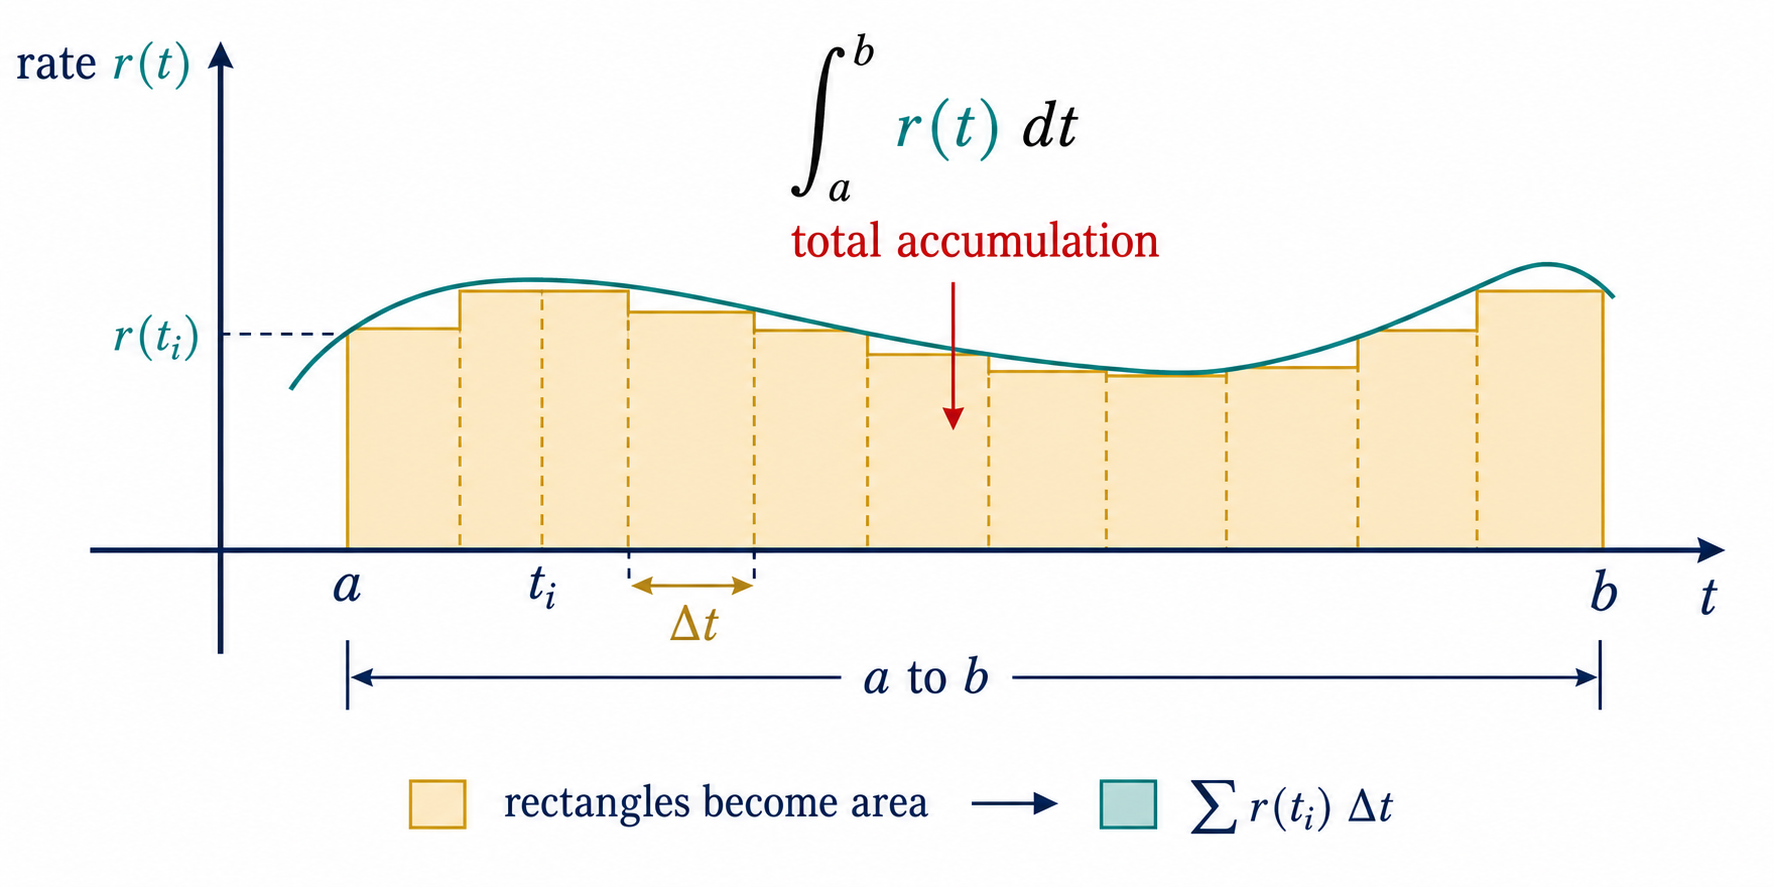
\includegraphics[width=0.95\linewidth]{imagegen-figures/ch08-integral-accumulation.png}
\caption{Integration accumulates many small rate-times-width contributions. Each rectangle contributes approximately \(r(t_i)\Delta t\). As the partition is refined, the rectangle sum approaches the shaded accumulated quantity \(\int_a^b r(t)\,dt\).}
\label{fig:ch08-integral-accumulation}
\end{figure}

\paragraph{Formal setup.}
Let \(r:[a,b]\to\mathbb{R}\) be a bounded function. A partition of \([a,b]\) is a finite list
\[
a=t_0<t_1<\cdots<t_n=b.
\]
Let \(\Delta t_i=t_i-t_{i-1}\), and choose a sample point \(t_i^\ast\in[t_{i-1},t_i]\). A Riemann sum is
\[
\sum_{i=1}^n r(t_i^\ast)\Delta t_i.
\]
If these sums approach a common value as the largest interval width goes to \(0\), that value is the definite integral:
\[
\int_a^b r(t)\,dt
=\lim_{\max_i\Delta t_i\to 0}
\sum_{i=1}^n r(t_i^\ast)\Delta t_i.
\]

The \emph{accumulation function} associated with \(r\) is
\[
A(t)=\int_a^t r(s)\,ds.
\]
It records the total accumulated from the starting point \(a\) up to the current point \(t\). If \(r\) is continuous and \(F'(t)=r(t)\), then the fundamental theorem of calculus states
\[
\int_a^b r(t)\,dt=F(b)-F(a).
\]
The variable \(t\) is the input variable, \(r(t)\) is the instantaneous contribution per unit \(t\), and \(dt\) marks the small width being accumulated.

\paragraph{Core intuition.}
Figure~\ref{fig:ch08-integral-accumulation} shows integration as a limit of structured approximation. At a coarse scale, rectangles give an approximate total. At a finer scale, the rectangles track the curve more closely. The limiting value is the integral.

The integral is the partner of the derivative. Derivatives start with accumulated values and ask for local rates. Integrals start with local rates and ask for accumulated values. The accumulation function \(A(t)\) sits between them: it stores total amount, and its derivative recovers the rate.

Common misconceptions include forgetting units, assuming all integrals are positive, and treating \(dt\) as decorative. The symbol \(dt\) tells us which variable is being accumulated over and carries the width of each small interval. Another common mistake is to confuse the integrand \(r(t)\), which is a rate, with the integral, which is a total.

This section extends sums from finite data vectors to continuous domains. It prepares continuous probability in Chapter 11 and Chapter 13, where probability densities integrate to probabilities and expectations are integrals of values weighted by densities.

\paragraph{Main theorem: fundamental theorem for accumulation functions.}
Let \(r:[a,b]\to\mathbb{R}\) be continuous, and define
\[
A(t)=\int_a^t r(s)\,ds.
\]
Then \(A\) is differentiable on \((a,b)\), and
\[
A'(t)=r(t).
\]

\emph{Proof sketch.} Start from the difference quotient for \(A\):
\[
\frac{A(t+h)-A(t)}{h}
=\frac{1}{h}\left(\int_a^{t+h}r(s)\,ds-\int_a^t r(s)\,ds\right).
\]
The shared accumulated part from \(a\) to \(t\) cancels, leaving
\[
\frac{A(t+h)-A(t)}{h}
=\frac{1}{h}\int_t^{t+h}r(s)\,ds.
\]
This is the average value of \(r\) on the short interval from \(t\) to \(t+h\). Because \(r\) is continuous, all values \(r(s)\) on that short interval become close to \(r(t)\) as \(h\to 0\). Therefore the average value approaches \(r(t)\), and
\[
A'(t)=r(t).
\]
In words: the derivative of total accumulated amount is the instantaneous rate of accumulation.

\paragraph{Worked examples.}
\emph{Small numerical example.} Approximate
\[
\int_0^2 t^2\,dt
\]
using four right-endpoint rectangles of width \(\Delta t=0.5\). The right endpoints are
\[
0.5,\qquad 1.0,\qquad 1.5,\qquad 2.0,
\]
so the sum is
\[
0.5\left(0.5^2+1^2+1.5^2+2^2\right)
=0.5(0.25+1+2.25+4)
=3.75.
\]
The exact integral is
\[
\int_0^2t^2\,dt=\left[\frac{t^3}{3}\right]_0^2=\frac{8}{3}\approx 2.67.
\]
The right-endpoint sum overestimates because \(t^2\) is increasing. Finer partitions reduce the error.

\emph{ML/neuroscience example.} Suppose a peri-stimulus firing-rate model is
\[
r(t)=20e^{-t/0.1}
\]
spikes per second for \(t\geq 0\). The expected spike count in the first \(0.2\) seconds after stimulus onset is
\[
\int_0^{0.2}20e^{-t/0.1}\,dt
=20\left[-0.1e^{-t/0.1}\right]_0^{0.2}
=2(1-e^{-2})
\approx 1.73.
\]
The function \(r(t)\) is an instantaneous rate; the integral is the accumulated expected count over the time window.

\paragraph{ML/DL/neuroscience connections.}
In statistical learning, the population risk is an integral over a data distribution:
\[
R(\theta)=\int \ell(f_\theta(x),y)\,p(x,y)\,dx\,dy.
\]
The empirical risk used in training is a finite-sample approximation to this integral. In neuroscience, firing rates integrate to expected spike counts, stimulus densities integrate to probabilities, and continuous-time signals are summarized by areas, energies, and averages. In probabilistic AI, expectations are integrals of values against probability densities.

\paragraph{Exercises.}
\begin{enumerate}[label=\textbf{8.3.\arabic*.}, leftmargin=*]
\item \textbf{Mechanical.} Compute \(\int_1^4(2t+3)\,dt\), and state the units of the answer if \(2t+3\) is measured in spikes per second and \(t\) in seconds.
\item \textbf{Proof or derivation.} Let \(A(t)=\int_0^t 3s^2\,ds\). Compute \(A(t)\) explicitly and verify that \(A'(t)=3t^2\).
\item \textbf{Numerical/computational.} Write pseudocode for the right-endpoint Riemann-sum approximation to \(\int_a^b r(t)\,dt\) using \(n\) equal subintervals. What inputs and outputs should the routine have?
\item \textbf{Interpretation.} A density \(p(x)\) integrates to \(1\) over all possible stimulus values. What does \(\int_c^d p(x)\,dx\) represent?
\item \textbf{Debug the misconception.} A student says, "An integral is always an area and therefore cannot be negative." Explain why \(\int_{-1}^1 x\,dx=0\) and \(\int_0^1(-2)\,dx=-2\).
\end{enumerate}

\subsection{8.4 Differential equations preview}

\paragraph{Motivating question.}
If we know the current state and the rule for its instantaneous rate of change, how do we recover the state trajectory over time?

\paragraph{Beginner setup.}
A \emph{differential equation} specifies a relationship involving an unknown function and its derivative. In an ordinary differential equation, or ODE, the unknown is a function of one independent variable, usually time. The central first-order form is
\[
\dot x(t)=f(x(t),t),
\qquad
x(t_0)=x_0.
\]
Here \(x(t)\) is the state, \(\dot x(t)=dx/dt\) is its rate of change, \(f\) is the rate rule, and \(x(t_0)=x_0\) is the initial condition.

The smallest useful example is exponential decay:
\[
\dot x(t)=-kx(t),
\qquad
x(0)=x_0,
\qquad
k>0.
\]
The rate is negative when \(x\) is positive, and its magnitude is proportional to the current state. The solution is
\[
x(t)=x_0e^{-kt}.
\]

ODEs solve the problem of converting local rules into global trajectories. The equation tells the state which direction to move at each instant; the initial condition tells us where to start.

What to keep in mind: a differential equation usually does not directly give \(x(t)\). It gives a rule for the slope of \(x(t)\). Solving or simulating the equation means finding a curve whose slope obeys that rule at every time.

\begin{figure}[htbp]
\centering
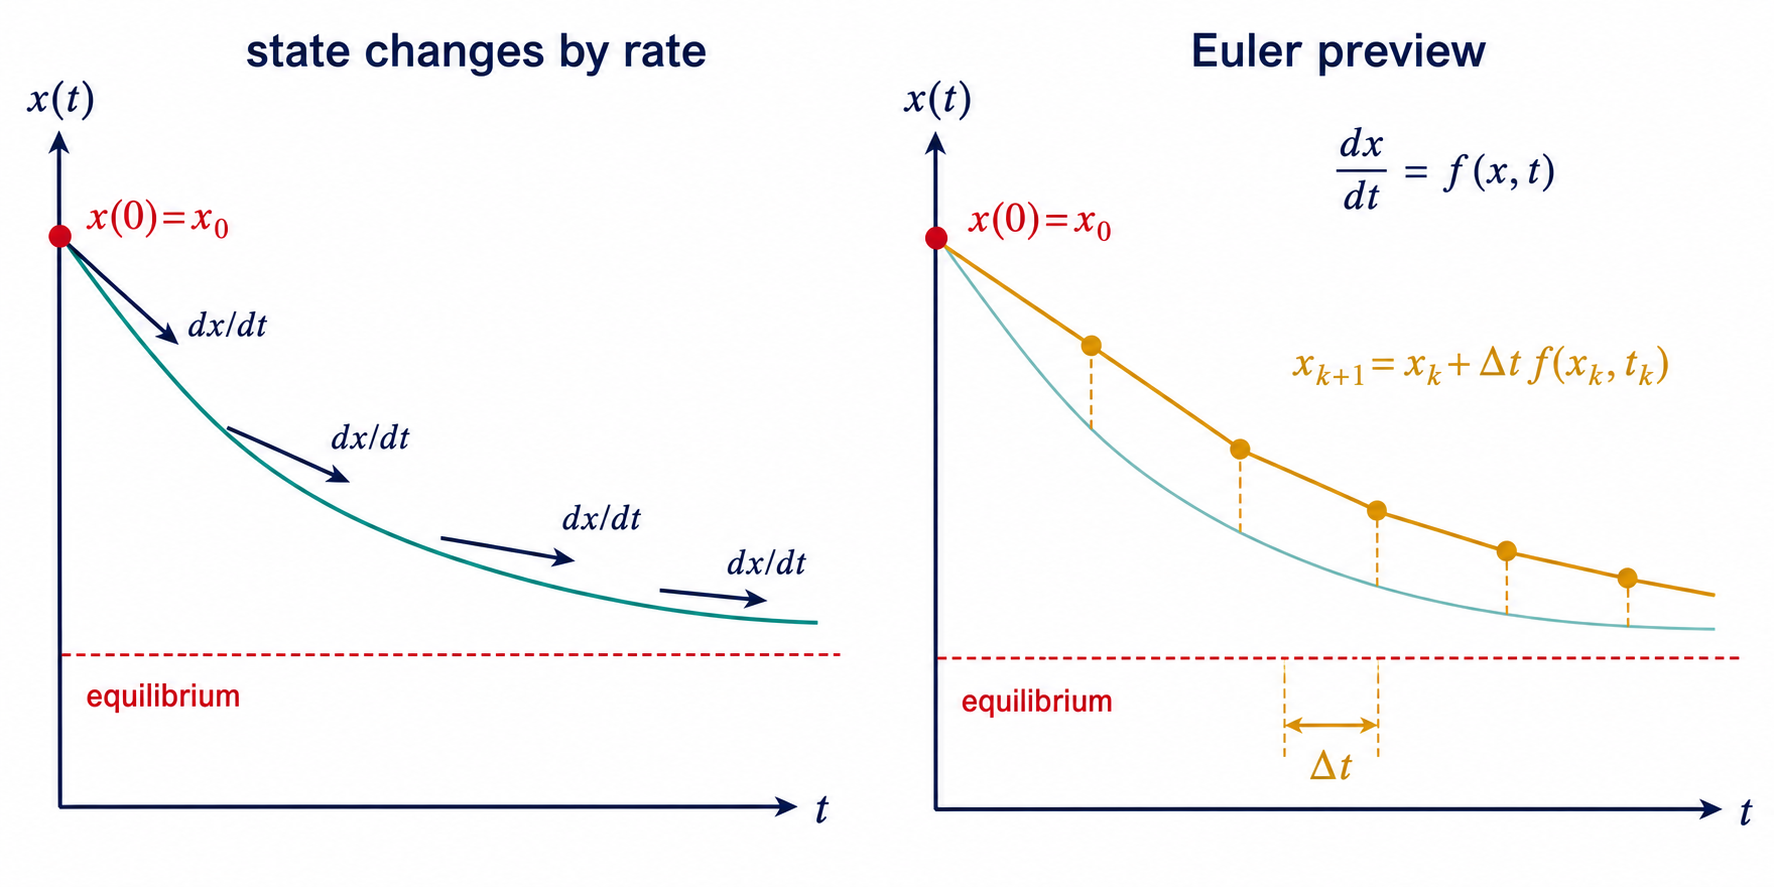
\includegraphics[width=0.95\linewidth]{imagegen-figures/ch08-ode-euler-preview.png}
\caption{An ODE specifies local rates, and a solution curve follows those rates from an initial condition. The decay trajectory approaches an equilibrium. Euler's method approximates the trajectory by repeatedly taking small straight steps \(x_{k+1}=x_k+\Delta t f(x_k,t_k)\).}
\label{fig:ch08-ode-euler-preview}
\end{figure}

\paragraph{Formal setup.}
For a scalar state, a first-order ODE has the form
\[
\frac{dx}{dt}=f(x,t),
\qquad
x(t_0)=x_0,
\]
where \(f:\mathbb{R}\times\mathbb{R}\to\mathbb{R}\) gives a rate. A solution is a differentiable function \(x(t)\) on an interval containing \(t_0\) such that
\[
x'(t)=f(x(t),t)
\]
for all times in the interval and \(x(t_0)=x_0\).

For a vector state \(x(t)\in\mathbb{R}^n\), the same notation becomes
\[
\dot x(t)=f(x(t),t),
\qquad
f:\mathbb{R}^n\times\mathbb{R}\to\mathbb{R}^n.
\]
This is the form used for recurrent neural dynamics, neural population state-space models, and continuous-time optimization.

An \emph{autonomous} ODE has no explicit time dependence:
\[
\dot x=f(x).
\]
An equilibrium \(x^\ast\) satisfies
\[
f(x^\ast)=0.
\]
If the state reaches \(x^\ast\), its instantaneous rate is zero, so it stays there.

Euler's method approximates an ODE by the update
\[
x_{k+1}=x_k+\Delta t\, f(x_k,t_k),
\qquad
t_{k+1}=t_k+\Delta t.
\]
This is local linearization applied repeatedly in time.

\paragraph{Core intuition.}
Figure~\ref{fig:ch08-ode-euler-preview} shows the central picture. At each point on the curve, the differential equation supplies a tangent slope. The solution is the curve whose tangent agrees with that slope everywhere. Euler's method replaces the curve by short tangent-line steps.

The decay equation \(\dot x=-kx\) is useful because the sign and magnitude are readable. If \(x>0\), then \(\dot x<0\), so \(x\) decreases. If \(x=0\), then \(\dot x=0\), so \(0\) is an equilibrium. If \(k\) is larger, the state decays faster.

Common misconceptions include treating \(\dot x=f(x,t)\) as an algebraic equation for \(x\), ignoring the initial condition, and assuming that an Euler simulation is exact. The initial condition is essential: many different trajectories may satisfy the same rate rule but start from different places. Numerical methods approximate solution curves, and their accuracy depends on the step size and the behavior of \(f\).

This preview uses derivatives from Section 8.2 and accumulation from Section 8.3. Later chapters will use the same local-to-global pattern for multivariable dynamics, neural state spaces, gradient flows, and stochastic processes.

\paragraph{Main derivation: exponential decay and Euler's approximation.}
Consider
\[
\dot x(t)=-kx(t),
\qquad
x(0)=x_0,
\qquad
k>0.
\]
Multiply both sides by \(e^{kt}\). Using the product rule,
\[
\frac{d}{dt}\bigl(e^{kt}x(t)\bigr)
=ke^{kt}x(t)+e^{kt}\dot x(t).
\]
Substitute \(\dot x(t)=-kx(t)\):
\[
\frac{d}{dt}\bigl(e^{kt}x(t)\bigr)
=ke^{kt}x(t)-ke^{kt}x(t)=0.
\]
Therefore \(e^{kt}x(t)\) is constant in time. At \(t=0\), this constant is \(x_0\). Hence
\[
e^{kt}x(t)=x_0,
\qquad
x(t)=x_0e^{-kt}.
\]

Euler's method applies the local linear update
\[
x_{k+1}=x_k+\Delta t(-kx_k)
=(1-k\Delta t)x_k.
\]
After \(m\) steps,
\[
x_m=(1-k\Delta t)^m x_0.
\]
When \(\Delta t\) is small and \(m\Delta t\approx t\), this discrete decay approximates the continuous solution \(x_0e^{-kt}\).

\paragraph{Worked examples.}
\emph{Small numerical example.} Let
\[
\dot x=-0.5x,
\qquad
x(0)=10.
\]
The exact solution is
\[
x(t)=10e^{-0.5t}.
\]
At \(t=4\),
\[
x(4)=10e^{-2}\approx 1.35.
\]
Euler's method with \(\Delta t=1\) gives
\[
x_{k+1}=0.5x_k,
\]
so the sequence is \(10,5,2.5,1.25,0.625\) at times \(0,1,2,3,4\). The approximation captures decay toward \(0\), but it undershoots the exact value because the step size is coarse.

\emph{ML/neuroscience example.} A leaky membrane-voltage model can be written as
\[
\tau\dot V(t)=-(V(t)-E_L)+RI(t),
\]
where \(V(t)\) is membrane voltage, \(E_L\) is leak reversal potential, \(I(t)\) is input current, \(R\) is resistance, and \(\tau\) is a time constant. The state is \(V(t)\). The right-hand side says that voltage is pulled back toward \(E_L\) while input current pushes it away. In a continuous-time recurrent neural network, a related state equation is
\[
\tau \dot h(t)=-h(t)+\phi(Wh(t)+Ux(t)),
\]
where \(h(t)\) is a hidden activity vector, \(\phi\) is a nonlinearity, and the matrices \(W,U\) define recurrent and input drive.

\paragraph{ML/DL/neuroscience connections.}
ODEs are the native language of continuous-time dynamics. In neuroscience they describe membrane voltage, synaptic currents, firing-rate dynamics, neural fields, and population state trajectories. In machine learning they appear in gradient flow \(\dot\theta=-\nabla L(\theta)\), neural ODEs, continuous normalizing flows, and dynamical systems models of sequence data. Euler's method also reveals a bridge to discrete-time computation: a residual network layer resembles one step of a dynamical system,
\[
h_{k+1}=h_k+\Delta t\,F(h_k,\theta_k).
\]

\paragraph{Exercises.}
\begin{enumerate}[label=\textbf{8.4.\arabic*.}, leftmargin=*]
\item \textbf{Mechanical.} Verify by differentiation that \(x(t)=4e^{-3t}\) solves \(\dot x=-3x\) with \(x(0)=4\).
\item \textbf{Proof or derivation.} For \(\dot x=ax\), \(x(0)=x_0\), derive the solution \(x(t)=x_0e^{at}\) using the product-rule method from the section.
\item \textbf{Numerical/computational.} Use Euler's method with \(\Delta t=0.25\) for \(\dot x=-2x\), \(x(0)=1\), from \(t=0\) to \(t=1\). List the four update values after \(t=0.25,0.5,0.75,1.0\).
\item \textbf{Interpretation.} In the membrane equation \(\tau\dot V=-(V-E_L)+RI(t)\), what happens to \(V(t)\) when \(I(t)=0\) and \(V(t)>E_L\)?
\item \textbf{Debug the misconception.} A student says, "The ODE \(\dot x=f(x,t)\) already tells us the value of \(x(t)\), so the initial condition is optional." Explain why the initial condition is necessary.
\end{enumerate}

\paragraph{Closing bridge.}
The chapter has moved from approach, to local change, to accumulation, to trajectories. The next chapter keeps the same ideas but replaces one input by many inputs. Limits become local behavior in \(\mathbb{R}^n\), derivatives become gradients and Jacobians, and second derivatives become Hessians that describe curvature. Later, integrals become expectations and ODEs become models of neural, optimization, and probabilistic dynamics.

\clearpage
